%
% LaTeX2e template for FIT2002
%


\documentclass[a4j,twocolumn]{ujarticle}
\usepackage[dvipdfmx]{graphicx}
\usepackage[dvipdfmx]{color}
\usepackage{ascmac}
\usepackage{url}



\makeatletter
\def\section{\@startsection{section}{1}{\z@}{2ex plus .2ex minus .2ex}%
{.5ex plus .2ex minus .2ex}{\large\bfseries}}
\def\thesection{\arabic{section}.}
\def\subsection{\@startsection{subsection}{1}{\z@}{.7ex plus .2ex minus .2ex}%
{.5ex plus .2ex minus .2ex}{\normalsize\bfseries}}
\def\thesubsection{\arabic{section}.\arabic{subsection}}
\def\thefootnote{\fnsymbol{footnote}}
\makeatother


\def\baselinestretch{0.8}

\setlength{\textheight}{23.5cm}%297-30-27 - 5
\setlength{\textwidth}{17.4cm}%210-18-18 - 10
%\setlength{\headheight}{0.0in}
\setlength{\headsep}{0.0in}
\setlength{\oddsidemargin}{-.9cm}%+3
\setlength{\evensidemargin}{-.9cm}%+3
\setlength{\columnsep}{7mm}


% local settings

% end of local settings


\begin{document}
    \pagestyle{empty}
    \thispagestyle{empty}

    \twocolumn[%
        \begin{center}
        {\Large 今学期作ったもの}
            \vspace{.5ex}

            {\Large\sffamily }\vspace{1ex}



            \large
            \mbox{}
            \hfil
            \setcounter{footnote}{2}
            {\bfseries Sociable Robots B1 澤田 開杜(sabaniki)}${}^\thefootnote$
            \hfil
            \setcounter{footnote}{3}
            \hfil
            \mbox{}

            \mbox{}
            \hfil
            {\sffamily}
            \hfil
            {\sffamily}
            \hfil
            \mbox{}
            \hfil

        \end{center}
    ]

    \setcounter{footnote}{2}
    \footnotetext{慶應義塾大学 環境情報学部}

\section{概要}
私が今学期製作した4つのプロダクトについて報告する。4つのプロダクトとは以下の表\ref{ProductsSem}に示した通りである。
毎月別のプロダクトに着手し、そのうち2つについては現在も開発を積極的に続けている。

\begin{table}[h]
    \caption{今学期製作したもの一覧}
    \label{ProductsSem}
    \centering
    \begin{tabular}{lcr}
        \hline
        着手時期 & 名前 \\
        \hline \hline
        4月 & ARplusR \\
        5月 & MTG-Shuffle \\
        6月〜 & IoT-Fam \\
        7月〜 & Over-Comment \\
        \hline
    \end{tabular}
\end{table}

\section{ARplusR}
\subsection{概要}
プロダクトの名前のARplusRとはAR+Robotを意味している。ARとロボットの組み合わせに興味が湧いたため、
プロトタイプとして、ARの入門も兼ねて作成したものである。
今回は実物のロボットを使わずに、ロボットも仮のものをAR上のオブジェクトで作成した。

\subsection{実装した機能}
以下に図\ref{ARRobotImage}として実際のアプリケーションのスクリーンショットを示す。
平面をアプリケーション上で検知し、その面に対して障害物に見立てた灰色の立方体を設置することができる。
すると、ロボットに見立てた黄色の立方体がその障害物を避けて前進するというものである。

\begin{figure}[h]
\centering
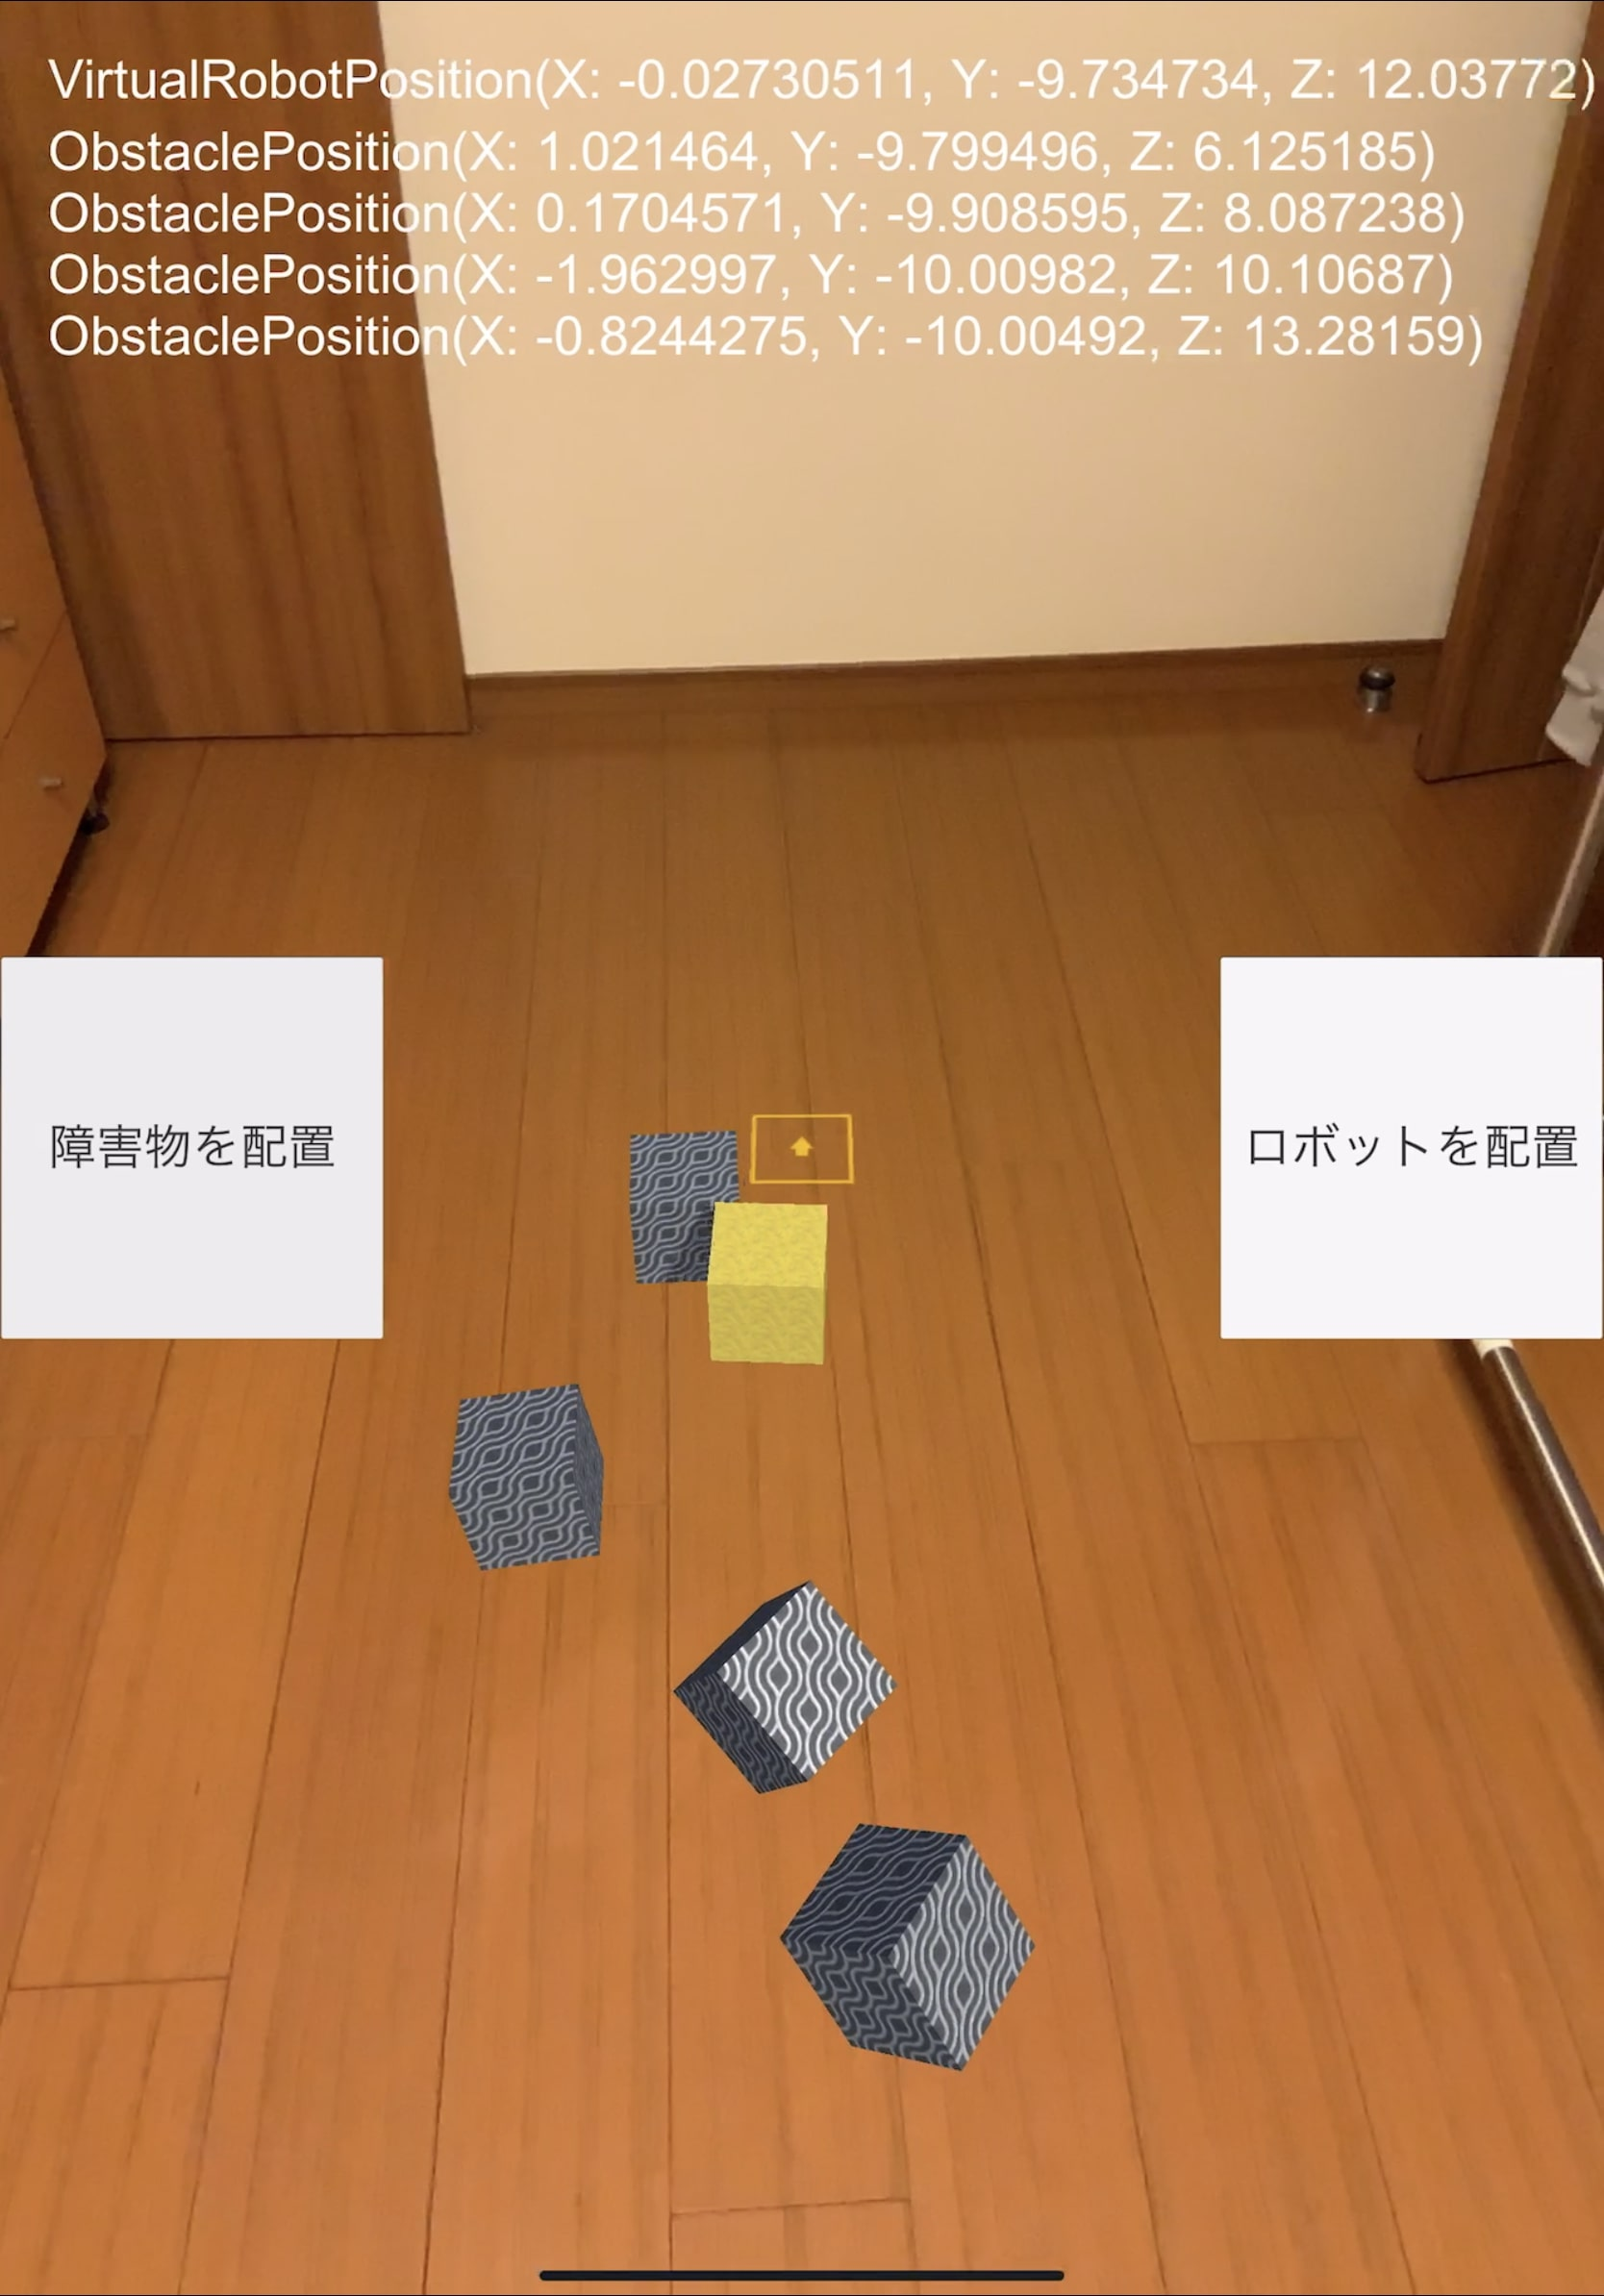
\includegraphics[width=3cm]{../assets/AR-Robot.jpg}
\caption{実際に作ったARアプリ}
\label{ARRobotImage}
\end{figure}

\subsection{展望}
今回は元々「ARを使うことで人間は視覚的にロボットに対して仮想的な情報を与えられる」
という部分に興味を持って取り組んだものだったが、
その特性を用いて具体的なプロトタイプを製作することはできなかった。
ロボットの進行方向をAR上で指示したり逆にロボットに侵入されたくない場所を指定するなどの案は出たが、
実現することはできなかった。
ARに興味がなくなったわけではなく、Apple Glassなどのまだ見ぬ新しいデバイスにも興味があるため、
今後も発展させていきたい。

\section{MTG-Shuffle}
\subsection{概要}
弊研究会では毎週火曜日に進捗報告とその週の目標を決めるグループ別のミーティングが行われる。
そのグループは院生をリーダとしてそこに均等になるように学部生が分かれるという形式であるが、
毎週のグループ分けが面倒であるという点があった。その問題を解決するべく、新人課題として取り組んだ。

\subsection{実装した機能}
以下に図\ref{MtgShuffleImage}としてアプリケーションのスクリーンショットを示す。
この図の通り、ランダムにグループを分ける機能を実装し、それを閲覧可能にしている。
また、ランダムにグループを分けるアルゴリズムは
院生や学部生の数が変化に依存しない仕組みになっている。
グループのリセットは一日に一度、誰か一人が行うことができる。
リセット限度を一日一度にしているため、
複数人がグループをリセットしてしまうことによる混乱が生じないよう工夫している。

\begin{figure}[h]
\centering
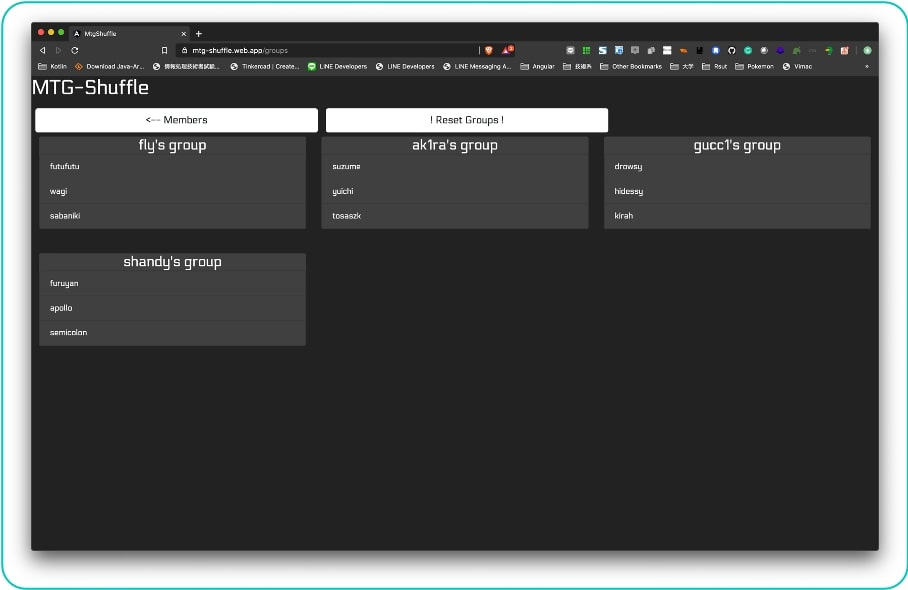
\includegraphics[width=5cm]{../assets/MTG-Shuffle.jpg}
\caption{MTG-Shuffle}
\label{MtgShuffleImage}
\end{figure}

\subsection{展望}
人数に依存しないアルゴリズムを考案するよりも前に
欠席者を除外してグループを作成する機能をつけるべきであったが、それがまだ実装されていない。
また、メンバーのCRUD機能も実装されておらず、いずれも仮のボタンが設置されているだけなので
なるべく早く実装する必要がある。また、完全にランダムにすると同じ人と当たりやすく感じることが
わかったため、同じ人と連続で当たりにくくなるようなアルゴリズムを考案し、実装する必要もある。

\section{IoT-Fam}
\subsection{概要}
最終的な完成形としては以下に図\ref{IoTFam}として示した通りである。
図ではSlackを使用しているが、家族LINEにIoTが参加し、
そこでのIoT同士の会話の中に人間が参加するというものである。
今現在のAlexaやGoogleHomeなどの中心的な存在があり、そこに対して人間が指示を出すと
各IoTが受動的で無機質にタスクをこなすという状態に対して私は疑問を感じたため製作を始めた。
\begin{figure}[h]
\centering
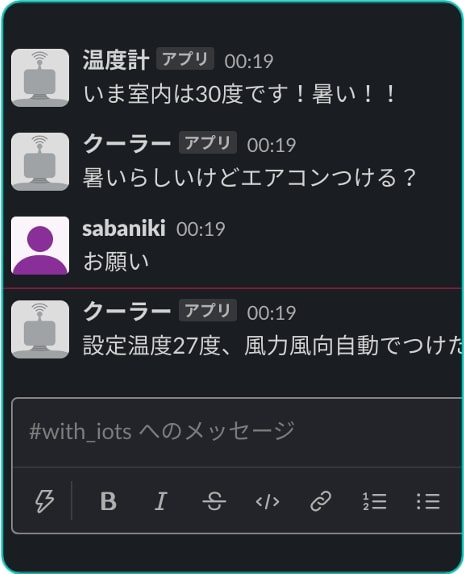
\includegraphics[width=5cm]{../assets/IoT-Fam.jpg}
\caption{IoT-Fam}
\label{IoTFam}
\end{figure}

\subsection{システム構成}
簡略的なシステム構成図を以下に図\ref{IoTFamSys}として示す。
中継サーバ(Raspberry Pi)を通してIoT(ESP)同士はJSON形式の情報をMQTT通信でやり取りし、
また、そのJSONデータは中継サーバ上で人間の会話に変換されSlackに送信される。
逆に人間の言葉からJSONを生成しESPとやり取りするアプリケーションもRaspberry Pi上で動作している。
JSON→会話の生成や会話→JSON生成については本格的な会話システムで処理しているわけではなく、
いわゆるif-thenの単純な仕組みで生成している。

\begin{figure}[h]
\centering
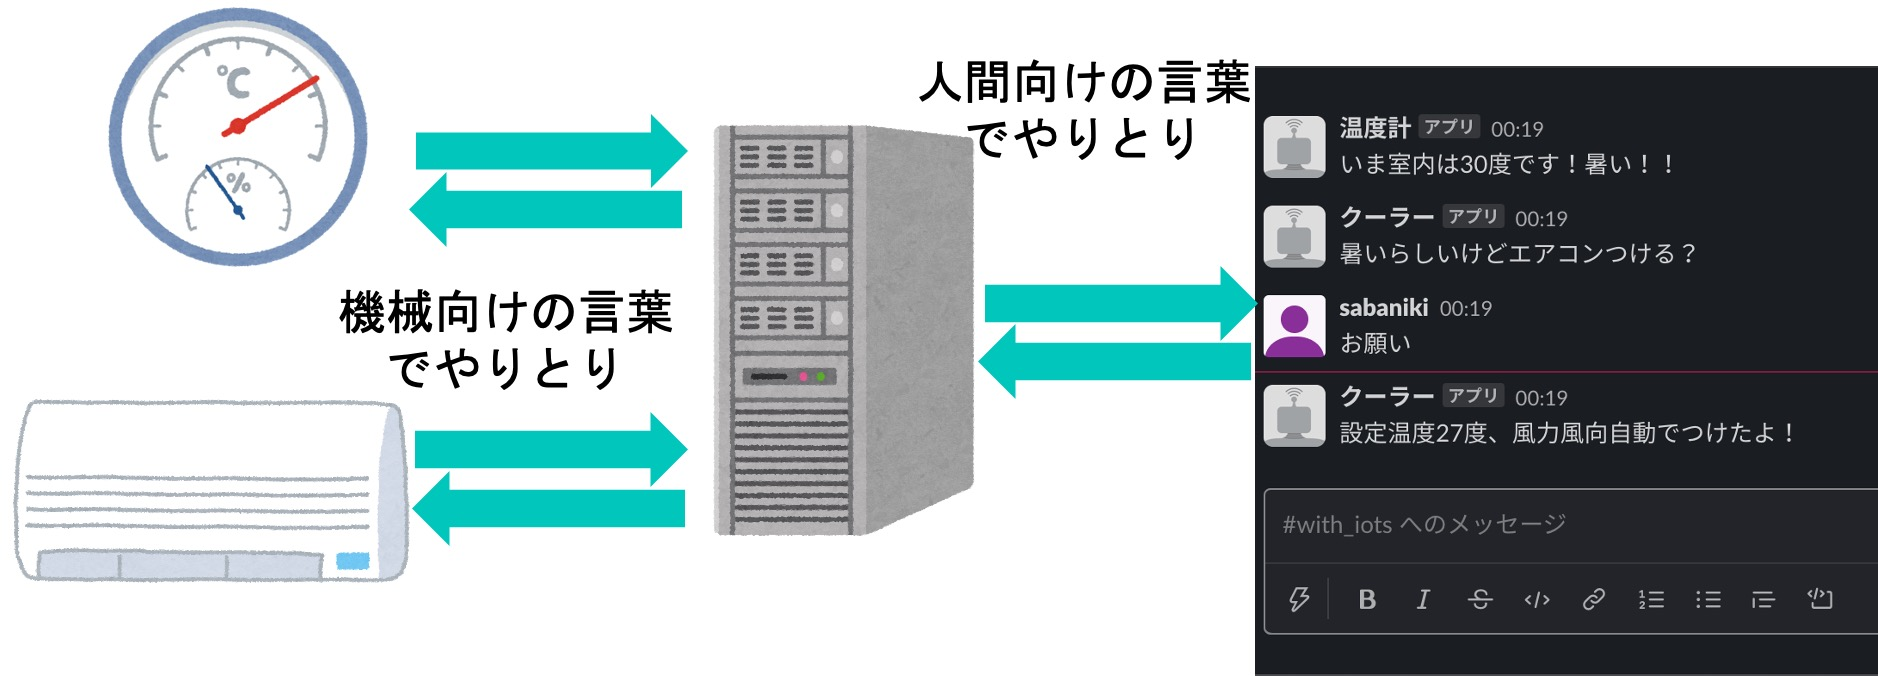
\includegraphics[width=8cm]{../assets/sys-strc.jpg}
\caption{IoT-Famシステム構成}
\label{IoTFamSys}
\end{figure}

\subsection{IoT部分}
今学期では図\ref{IoTFam}で示したシチュエーションを満たすために温度計デバイス、エアコン制御
を作成した。

\subsubsection{温度計}
温度計デバイスの実物の画像を以下に図\ref{TempImage}として示す。
湿度も取得可能なセンシングモジュールを採用したため、温度だけでなく当初は計測予定でなかった湿度も
取得可能となった。値を取得しMQTT通信で送信することは可能だが、接続が不安定になることが多々ある。
専用のソケットの代わりにジャンパワイヤで強引に接続していることが原因であると考えられる。

\begin{figure}[h]
\centering
\includegraphics[width=5cm]{../assets/temp.JPG}
\caption{温度計デバイス}
\label{TempImage}
\end{figure}

\subsubsection{エアコン}
エアコン制御デバイスの実物の画像を以下に図\ref{AirConImage}として示す。
このデバイスを使用し、私の部屋に設置されているアイリスオーヤマ製のエアコンの赤外線リモコンを解析して
起動させることができた。無線での操作も実現できたが赤外線LEDの指向角や放射強度について深く考えずに購入
してしまったため、角度を調整したり近づけたりしないと現状ではうまく起動させることができない。
また、仮に起動のみを行いたい場合でもリモコンから送られる信号には温度や風量の情報も含まれており、
信号のどの部分が温度にあたりどの部分が風量に当たるかなどの解析はできていないため、解析は部分的にしか
実現していない。

\begin{figure}[h]
\centering
\includegraphics[width=5cm]{../assets/AirCon.JPG}
\caption{エアコン制御デバイス}
\label{AirConImage}
\end{figure}

\subsection{展望}
今学期では図\ref{IoTFam}で示したシチュエーションを実現することはできたが、
このシチュエーションのみしか実装できなかったため、当初の”IoT同士の会話の中に参加する”という感覚を
得ることはできなかった。また、擬人化してある部分が特徴の一つであるプロダクトだが、私自身が
あまり擬人化してあることに意味を感じなかった。しかし、IoTデバイス同士のやりとりに参加するという部分は
各デバイスが持っている情報を人間が確認しやすく利便性があると個人的に感じたため、その部分をより生かして
いきたい。Twitterのように各デバイスが自分の持っている情報を発信するようなSNS的な仕組みも面白いのでは
ないかと考えている。

\section{Over-Comment}
\subsection{概要}
このプロダクトはZoomやWebex上でニコニコ動画のようなコメントシステムを再現するというものである。
ZoomやWebexでのコメントは通知が控えめで気が付きにくく、送信者側も相手に届いてるいるという確証を
持ちにくいと私は感じた。ニコニコ動画のようなコメントシステムなら、追いきれない程の量でなければ
コメントが目に入らないということは少ないと考え、この形式を採用した。今回はコメントを表示する
デスクトップアプリケーション、コメントの送信や履歴の閲覧などを行うためのWebアプリケーション
の二つを作成した。

\subsection{システム構成}
以下に図\ref{sys-strc-oc}として簡略的なシステム構成図を示す。Webアプリケーション部分はAngularを用いて開発し、Firebase上で
ホスティングしている。Webアプリケーション部分でコメントをデータベース(Firebase Realtime Database)に送信すると、
そのデータベースの変更を検知してデスクトップアプリケーション側でコメントを受け取るという仕組みになっている。また、Webアプリケーション
のコメントの履歴機能についても同じ様にデータベースの変更を検知し、リアルタイムに履歴が反映されるようになっている。

\begin{figure}[h]
\centering
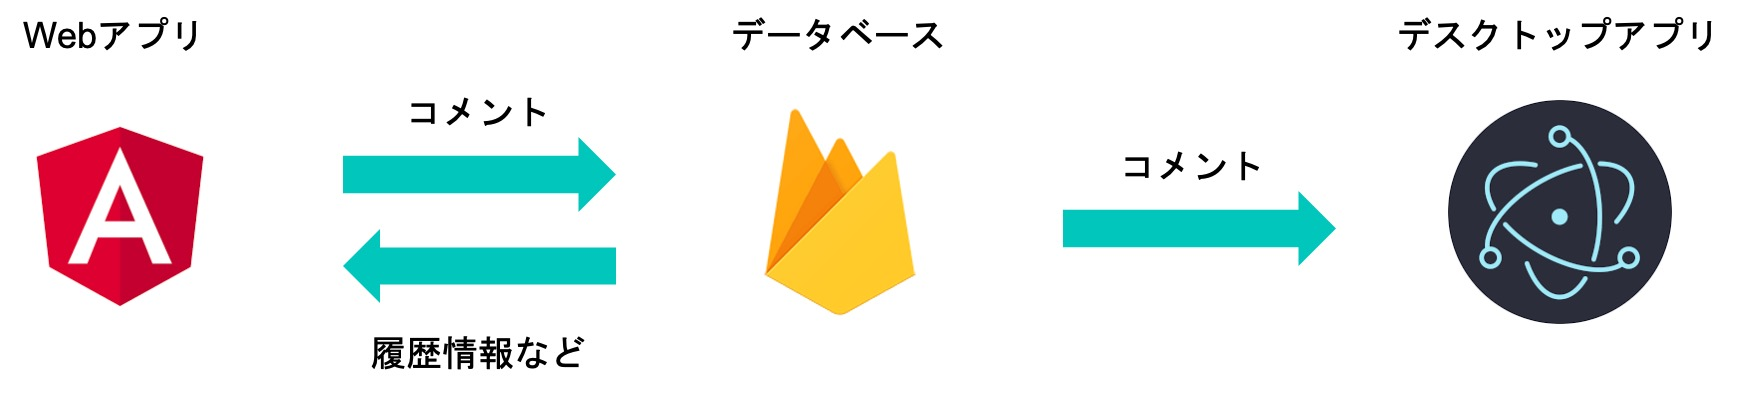
\includegraphics[width=8cm]{../assets/sys-strc-oc.jpg}
\caption{Over-Commentシステム構成}
\label{sys-strc-oc}
\end{figure}

\subsection{実装した機能}

\subsubsection{デスクトップアプリケーション}
以下に図\ref{dsk-app}として実際にデスクトップアプリケーションが稼働している様子を示す。
利便性を考え、このアプリケーションはOSに依存せず実行可能なElectronで作成した。
透明でマウスイベントを無視するウィンドウ上にコメントを右から左に流すようになっているため、
ZoomやWebexなどの他のアプリケーションにオーバーラップしつつ、その別のアプリケーションを操作することができる。
受け取ったコメントは一度キューに保存し1秒ごとにデキューして表示することで、一度に多くのコメントが投稿された際に
処理が上がりすぎないようにしている。 マウスイベントを無視する仕様にしている関係上このアプリケーションに機能を多くもたせると操作しにくい
と考え、多くをWebアプリケーションに担わせる設計とした。

\vspace{3cm}
\begin{figure}[h]
\centering
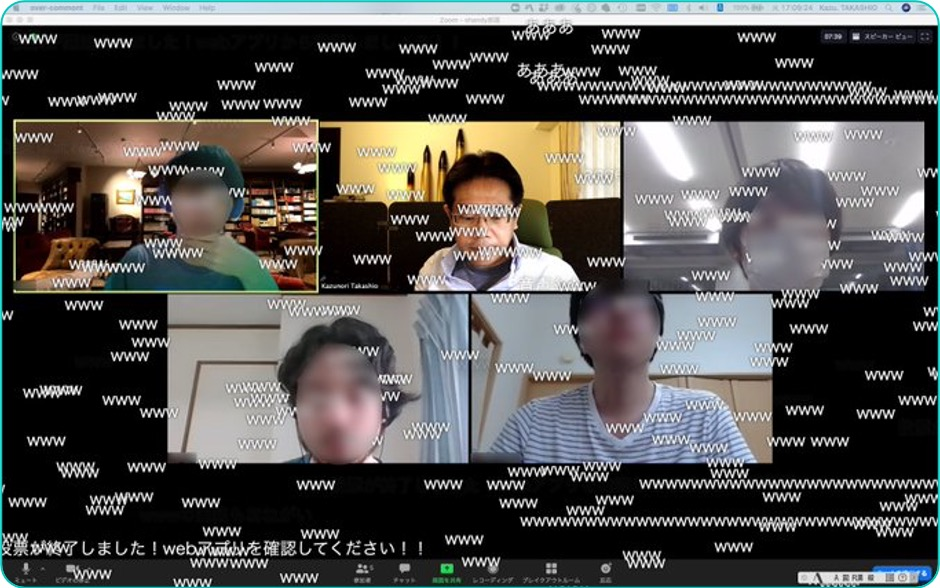
\includegraphics[width=5cm]{../assets/dsk-app.jpg}
\caption{デスクトップアプリケーション}
\label{dsk-app}
\end{figure}

\subsubsection{Webアプリケーション}
以下に図\ref{web-app}としてWebアプリケーションのスクリーンショットを示す。
このWebアプリケーションはAngularで作成した。単にコメントを送信できるだけでなく、コメントの色やフォントサイズを変えられたり
履歴を確認したりすることができる。また、コメントシステムだけでなくアンケートを実施することもできる。また、簡単にリアクションを送れる
方法としてwwwと書かれたボタンとcrapと書かれたボタンを実装した。wwwと書かれたボタンは押すと笑いを意味するwwwというコメントを送信する
ことができ、crapと書かれたボタンは押すと拍手を意味する88888888というコメントが送信される。このcrapに関しては単にコメントが流れる
だけでなく拍手の音も再生される。自分が発表を行った際に相手のリアクションがわかりにくかったり逆に聞く方もオフライン時のような音を伴った
リアクションを送りにくいという点が問題だと感じたためこの機能を実装した。また、このアプリケーションはウィンドウを小さくして使用する
ことを想定しており、特にスマートフォンからの操作を意識して作成した。特に笑いや拍手をスマホを片手にリモコン感覚で送信してもらう
シチュエーションを想定していたが、実際は自分を含めてパソコンだけで使う人が多い結果となった。

\begin{figure}[h]
\centering
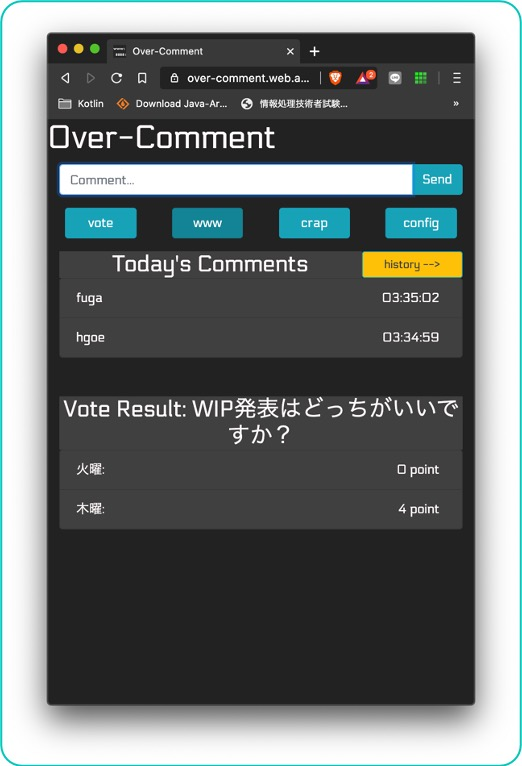
\includegraphics[width=3cm]{../assets/web-app.jpg}
\caption{Webアプリケーション}
\label{web-app}
\end{figure}

\bibliographystyle{junsrt}
\bibliography{bib.bib}



\end{document}
